%
% File acl2019.tex
%
%% Based on the style files for ACL 2018, NAACL 2018/19, which were
%% Based on the style files for ACL-2015, with some improvements
%%  taken from the NAACL-2016 style
%% Based on the style files for ACL-2014, which were, in turn,
%% based on ACL-2013, ACL-2012, ACL-2011, ACL-2010, ACL-IJCNLP-2009,
%% EACL-2009, IJCNLP-2008...
%% Based on the style files for EACL 2006 by 
%%e.agirre@ehu.es or Sergi.Balari@uab.es
%% and that of ACL 08 by Joakim Nivre and Noah Smith

\documentclass[11pt,a4paper]{article}
\usepackage[hyperref]{acl2019}
\usepackage{times}
\usepackage{latexsym}
\usepackage{graphicx}
\usepackage{amsmath}
\usepackage{amssymb}
\usepackage{booktabs}
\usepackage{url}

%\aclfinalcopy % Uncomment this line for the final submission
%\def\aclpaperid{***} %  Enter the acl Paper ID here

%\setlength\titlebox{5cm}
% You can expand the titlebox if you need extra space
% to show all the authors. Please do not make the titlebox
% smaller than 5cm (the original size); we will check this
% in the camera-ready version and ask you to change it back.

\newcommand\BibTeX{B\textsc{ib}\TeX}

\DeclareMathOperator{\softmax}{softmax}
\DeclareMathOperator{\sigmoid}{sigmoid}

\definecolor{Orange}{RGB}{255,140,0}
\definecolor{Blue}{RGB}{0,191,255}
\newcommand{\ek}[1]{\textcolor{Orange}{[ek: #1]}} 
\newcommand{\cp}[1]{\textcolor{Blue}{[cp: #1]}} 

\newcommand{\aout}{\mathbf{a_{\text{out}}}}

% \title{Predicting guilt judgments from crime stories}
\title{Attention Weights as a Window into How Crime Narratives Shape Subjective Assessments of Guilt}

\author{Elisa Kreiss \\
  Department of Linguistics \\
  Stanford University \\
  \texttt{ekreiss@stanford.edu} \\\And
  Judith Degen \\
  Department of Linguistics \\
  Stanford University \\
  \texttt{jdegen@stanford.edu} \\\And
  Christopher Potts \\
  Department of Linguistics \\
  Stanford University \\
  \texttt{cpotts@stanford.edu}\\}

\date{}

\begin{document}
\maketitle
\begin{abstract}
  Neural network attention mechanisms have led to performance gains on a wide variety of tasks in natural language understanding, and they have also provided clues as to how these complex networks represent the language they process, opening up new avenues for linguistic investigation. In this spirit, we apply neural networks with attention to the task of modeling human judgments about guilt based on short crime narratives. The networks are successful at the task, and probing their attention weights helps illuminate the ways in which they make use of markers of certainty and uncertainty in different crime narratives, suggesting new hypotheses about how crimes might be more effectively reported in the news media.
\end{abstract}

\section{Introduction}

%\ek{update according to framing proposal in email}

Deep learning models are increasingly applied to language tasks not only to develop technologies but also to derive new insights into language use. These more scientific applications raise the question of whether the models are processing data in a motivated way; their ``black box'' nature is often an obstacle to answering this question \citep{Alishah-etal:2019}. Recently, attention mechanisms, which capture the strength of association between components of these networks \citep{bahdanau2014neural,luong-etal-2015-effective}, have not only improved performance, but also increased interpretability, potentially opening the door to new linguistic applications of these models (\ek{paper that challenges this idea a little: }\cite{Serrano:2019}).

In this paper, we apply neural networks with attention to a task that has both linguistic and societal import: predicting whether the reader of a short narrative crime report will conclude that the main subject is guilty or innocent. Our networks achieve strong performance on this task, as defined by the dataset of \citet{Kreiss:2019}, which leads us to explore their learned parameters by inspecting how they make predictions for new, carefully controlled examples. We find that the networks make robust use of markers of certainty and uncertainty, as well as discourse connectives that signal contrast. In addition, by systematically removing this language from test examples, we see that these markers have a large impact where the evidence is weak but have little or no impact where the evidence is strong. To the extent that humans adopt similar reading strategies, this can inform how the news is reported, in that it gives us insights into the contribution of words like \emph{allegedly} and \emph{possibly} in shaping readers' construal of newspaper articles \citep{Erickson-etal:1978,jensen2008scientific}.


\section{Related Work}

Our work draws on prior research concerning the relationship between language and assesments of guilt, as well as work seeking to use neural networks to inform linguistic theory.


\subsection{Predicting Guilt}
% 1. Topic sentence (e.g., "There is extensive prior literature on how linguistic markers influence perceptions of guilt").
The challenge of predicting guilt judgments from text sources has not yet received a lot of attention. 
% 2. Basically a list of papers falling under the topic, with basic details about what the work does.
However, \citeauthor{Fausey:Boroditsky:2010} show that using agentive language increases blame and financial liability judgments people make. Their results suggest that even subtle linguistic changes in crime reports can shape people's judgments of the events.
More recent work has focused on predicting guilt verdicts from the Supreme Courts in the Philippines \citep{virtucio2018predicting} and Thailand \citep{kowsrihawat2018predicting} on the basis of facts presented and legal texts. \citeauthor{kowsrihawat2018predicting} argue for a recurrent neural network with attention to make these predictions. This work is not concerned with the linguistic basis of subjective moral guilt judgments, but Court guilt verdicts on the basis of a given law text. 
% 3. A final section explaining how the above relates to the current paper.
It is our goal to train a network on subjective guilt ratings and then probe its parameters with respect to their linguistic basis.

\subsection{Interpretation of Hedges}

% 1. Topic sentence (e.g., "There is extensive prior literature on how linguistic markers influence perceptions of guilt").
In the literature, researchers have categorized and labeled (un)certainty markers in numerous ways, e.g., \citep{lakoff1972hedges, prince1982hedging, brown1987politeness}. For a summary, we refer readers to \citealt{fraser2010pragmatic}. 
In this work, we use ``hedge'' broadly, as an umbrella term for all subclasses of uncertainty markers, including any marker that introduces uncertainty ``within the propositional content'' (e.g., ``His feet were \textbf{sort of} blue'') or ``in the relationship between the propositional content and the speaker'' (e.g., ``\textbf{I think} his feet were blue'').\cp{Where do the quoted phrases come from? Fraser?}

% 1. Topic sentence
There is extensive prior literature on how hedges affect perceptions of the speaker and proposition \citep{Erickson-etal:1978, durik2008effects, bonnefon2006tactful, rubin:2007:ShortPapers, jensen2008scientific, ferson2015natural}.  The resulting picture is highly varied. 
% 2. Basically a list of papers falling under the topic, with basic details about what the work does.
These studies suggest that hedges affect people's judgments of credibility in differing ways. For example, an increase in the number of hedges decreases the credibility of witness reports \citep{Erickson-etal:1978}, but, at the same time, increases the trustworthiness of journalists and scientists \citep{jensen2008scientific}. Additionally, the interpretation of hedges is very context dependent \citep{bonnefon2006tactful,durik2008effects,ferson2015natural} and shows high individual variation \citep{rubin:2007:ShortPapers,ferson2015natural}. 
% 3. A final section explaining how the above relates to the current paper.
We investigate how neural network predictions about human judgments change when we manipulate the presence of those hedges in crime stories.

<<<<<<< HEAD
In addition, computational and theoretical work on veridicality has revealed that not all hedges serve merely to reduce speaker commitment. For instance, attitude predications like ``The company reported S'' and ``They said S'' are often used to convey evidence sources. In such utteraces, the speaker might wish to appear fully commited to the embedded content ``S'' \citep{Simons07,deMarneffe:Manning:Potts:2012,White:Rawlins:2018,White-etal:2018}. \citet{vonFintel:Gillies:2010} show that similarly evidential readings arise for epistemic ``must''. These findings show how complex these markers are pragmatically and highlight the value of usage-based studies of them.


\subsection{Gaining Linguistic Insights Through Neural Networks}

Neural networks were originally motivated largely by questions in cognitive science \citep{pater2019generative}, especially concerning issues of representation and learning (e.g., \citep{rumelhart1986learning,tesar2000learnability}). Today, they are more closely associated with engineering efforts, but there is increasing interest in returing to these models' cognitive motivations and in using them to try to gain insights about linguistic phenomena. The incredible representational power of these networks has long been an obstacle to such work, but recent efforts are overcoming these obstacles. For instance, \citet{N16-3020} and \citet{Koh:Liang:2017} develop methods for probing complex models to understand which features are guiding their predictions. Attention weights are increasingly playing a role in such efforts. For instance, \citet{jawahar-etal-2019-bert} and \citet{tenney-etal-2019-bert} present evidence that BERT language models systematically encode core aspects of linguistic structure. We present a similar argument here, but focused on usage-based patterns. Finally, \citet{linzen-etal-2016-assessing} explicitly argue for applying methods from psycholinguisics to trained neural networks, treating them as participants whose performance we can observe and learn from (see also \citealt{gulordava-etal-2018-colorless,Futrell-etal:2019}).



% . For an overview on the interplay of generative linguistics and neural networks, we recommend \cite{pater2019generative}. Other work uses artificial language constraints on those networks to investigate language universals \ek{cite Greenberg, Michael Hahn}.\ek{more? dependency structure in BERT, Kevin Clark 2019; treat nns as human subjects, Levy and Futrell 2019}
% % 3. A final section explaining how the above relates to the current paper.
% In this work we pick out a particular feature of language use (hedges) and investigate model predictions in their presence and absence.
=======
\subsection{Linguistic basis in neural networks}

% 1. Topic sentence.
% people have used attention weights to show that the network has learned something that seems aligned with what we think we know about language
Neural networks have been shown to achieve high performances on various NLP tasks, such as sentiment analysis \cite{Socher:2013,Devlin:2018} and translation \cite{bahdanau2014neural}. A growing amount of literature has tried to gain linguistic insight from those neural networks \citep{belinkov2019analysis}.
% 2. Basically a list of papers falling under the topic, with basic details about what the work does.
For example, neural networks seem to learn some basic syntactic structures. \citeauthor{futrell-etal:2019-neural-language-models} find evidence for basic incremental syntactic state representations by treating neural network outputs like human subjects \citep{linzen2016assessing}. A vast amount of recent literature finds that that contextual word embedding models like BERT \citep{Devlin:2018} have structural information encoded \citep{jawahar-etal-2019-bert, Tenney:2019, clark2019what}. \citeauthor{clark2019what} find indications that particular attention heads in BERT specialize to specific aspects of syntax. Generally attention weights have been used for the analysis of neural language models, for example, in tasks such as NLI \citep{rocktaschel2015reasoning, yin2016abcnn}, sentiment analysis and \citep{wang2016attention, liu2017attention} summarization \citep{rush-etal-2015-neural, allamanis2016convolutional}. In these studies, attention weights seem to align with natural language intuitions and are used as windows into what guides predictions.
% 3. A final section explaining how the above relates to the current paper.
In this work we visualize the attention weights and probe the model outputs to gain insight into what the model learns for guilt prediction.
>>>>>>> origin/master


% ####

% TODO: move to model section
% The central challenge is to find a promising neural network architecture that can extract relevant features of an input paragraph. This can then be used to predict a value that represents a guilt judgment.

% \paragraph{Word embeddings}
% There are a variety of systems that investigate how to find meaningful word representations. In the literature, GloVe word embeddings \citep{Pennington:2014} have been widely used to represent word meanings. Those embeddings are context-independent, i.e., each word only has one respective vector representation independent of the context it occurs in.

% More recent advances in word embeddings aim to provide context-sensitive word representations to obtain richer and more informative word meaning representations (e.g., ELMo \cite{Peters:2018} and BERT \cite{Devlin:2018}). The BERT word embedding model is a Transformer based network which incorporates the context before and after the critical word to obtain a word representation. \citeauthor{Devlin:2018} report that using these embeddings boosts performance in all of the 11 natural language tasks it was trained on compared to previous systems.

% \paragraph{Paragraph embeddings}
% While word embeddings are useful, we need to arrive at a meaningful \textbf{paragraph} representation for our purposes. In other words, the word embeddings need to be combined in a meaningful way to arrive at a more complex representation.

% For short phrases, bidirectional LSTMs \cite{Hochreiter:1997,Schuster:1997,Graves:2005} have been shown to be a useful tool. However, they have difficulty resolving long-term dependencies, which is why their performance decreases with longer input paragraphs \cite{Hochreiter:2001}. \cite{Vaswani:2017} developed am attention mechanism to resolve these issues in Transformers. However, a similar principle can be applied to LSTM architectures as well.

% \cite{Lin:2017} introduce a bidirectional LSTM with self-attention that receives word embeddings as an input and outputs a paragraph representation. The bidirectional LSTM receives the GloVe embeddings of the paragraph as input. The self-attention layer is the weighted sum of all of the LSTM's hidden states. But instead of using a single weighted sum to arrive at a vector, they suggest to perform this multiple times with different weight vectors to arrive at an attention matrix. Furthermore, they introduce a penalization term which ensures that each attention vector in this attention matrix focuses on different semantic features of the input paragraph. Which semantic features are more important than others can in turn be learned again, dependent on the task it needs to solve. \citeauthor{Lin:2017} report that the model outperforms previous models in author profiling, sentiment classification and textual entailment.

\section{Dataset}
<<<<<<< HEAD
For training and testing the model, we use the Annotated Iterated Narration Corpus (AINC) collected by \citet{Kreiss:2019}.\footnote{\url{https://github.com/elisakreiss/iterated_narration}} The corpus was created for investigations on how news stories change when they are propagated from one person to another.

First, the authors created five stories of approximately 850 words, which are called the \emph{seed} stories. All of them report a crime and an arrest of one or more suspects. Each of these five seed stories exists in a weak and a strong evidence condition. The stories are identical up to the last phrase, which then either raises doubts about the arrest or emphasizes its validity. For example, if a suspect was arrested on the basis of camera footage, this footage was described as being of ``very poor quality'' in the weak evidence condition and ``very high quality'' in the strong evidence condition. Table~\ref{tab:examplestory} provides a complete example.

Each story was given to a participant who was asked to read and afterwards reproduce it. The reproduced story was then given to the next participant who again reproduced it. This pattern was repeated for 5 generations of participants. The data collection therefore followed the transmission-chain paradigm, introduced by \cite{Bartlett:1932}. Following this schema, each story and condition was reproduced in 5 chains over 5 generations, resulting in 250 reproductions, and therefore 260 stories overall. % (see Figure~\ref{fig:corpus-overview}).

\begin{table*}
\centering
\begin{tabular}{p{.45\textwidth} p{.45\textwidth}}
  \toprule
  \multicolumn{2}{p{0.925\textwidth}}{In late December 2017, a couple in Iowa was checking on their 50 beehives when they discovered a tragic scene. The hives had been overturned and hacked apart, and the equipment had been thrown out of the shed and smashed. This destruction caused the death of about half a million bees and approximately \$60,000 in property damage. Nearly three weeks later, police arrested two boys (12 and 13 years old) who, allegedly, were responsible for the damage. The charges against them include criminal mischief, burglary, and offenses to an agricultural animal facility. Since they are still minors, they will be charged in juvenile court where they face up to 10 years in prison and fines of up to \$10,000 if convicted.}\\ 
  \midrule
  (\emph{strong evidence condition}) & (\emph{weak evidence condition})  \\
  Police officials explained that the investigation is still in progress, but the evidence so far overwhelmingly speaks to the guilt of the suspects.  & Police officials explained that the investigation is still in progress, and the evidence so far doesn't warrant rushed conclusions about the guilt of the suspects. \\ 
  \bottomrule
\end{tabular}
\caption{Example of a seed story used in Exp.~1. \cp{I copied this over from the CogSci paper. We should select a different one, though -- again trying to balance using this corpus as a public resource and avoiding a problem with anonymous review.}}
\label{tab:examplestory}
\end{table*}

=======
For training and testing the model, we use the Annotated Iterated Narration Corpus (AINC) collected by \cite{Kreiss:2019}. \cp{I think we have to make this corpus public and include the URL to download it, else this will be seen as an indirect violation of anonymity.}\ek{I see, that makes sense. Chris/Judith: What is a good way to make the corpus public? Github?} The corpus was created for investigations on how news stories change when they are propagated from one person to another. First the authors created five stories of approximately 850 words, which are called the \emph{seed} stories. All of them report a crime and an arrest of one or more suspects. Each of these five seed stories exists in a weak and a strong evidence condition. The stories are identical up to the last phrase, which then either raises doubts about the arrest or emphasizes its validity. For example, if a suspect was arrested on the basis of camera footage, this footage was described as being of ``very poor quality'' in the weak evidence condition and ``very high quality'' in the strong evidence condition. Each story was given to a participant who was asked to read and afterwards reproduce it. The reproduced story was then given to the next participant who again reproduced it. This pattern was repeated for 5 generations of participants. The data collection therefore followed the transmission-chain paradigm, introduced by \cite{Bartlett:1932}. Following this schema, each story and condition was reproduced in 5 chains over 5 generations, resulting in 250 reproductions, and therefore 260 stories overall. % (see Figure~\ref{fig:corpus-overview}).
>>>>>>> origin/master

% \begin{figure}[t!]
% 	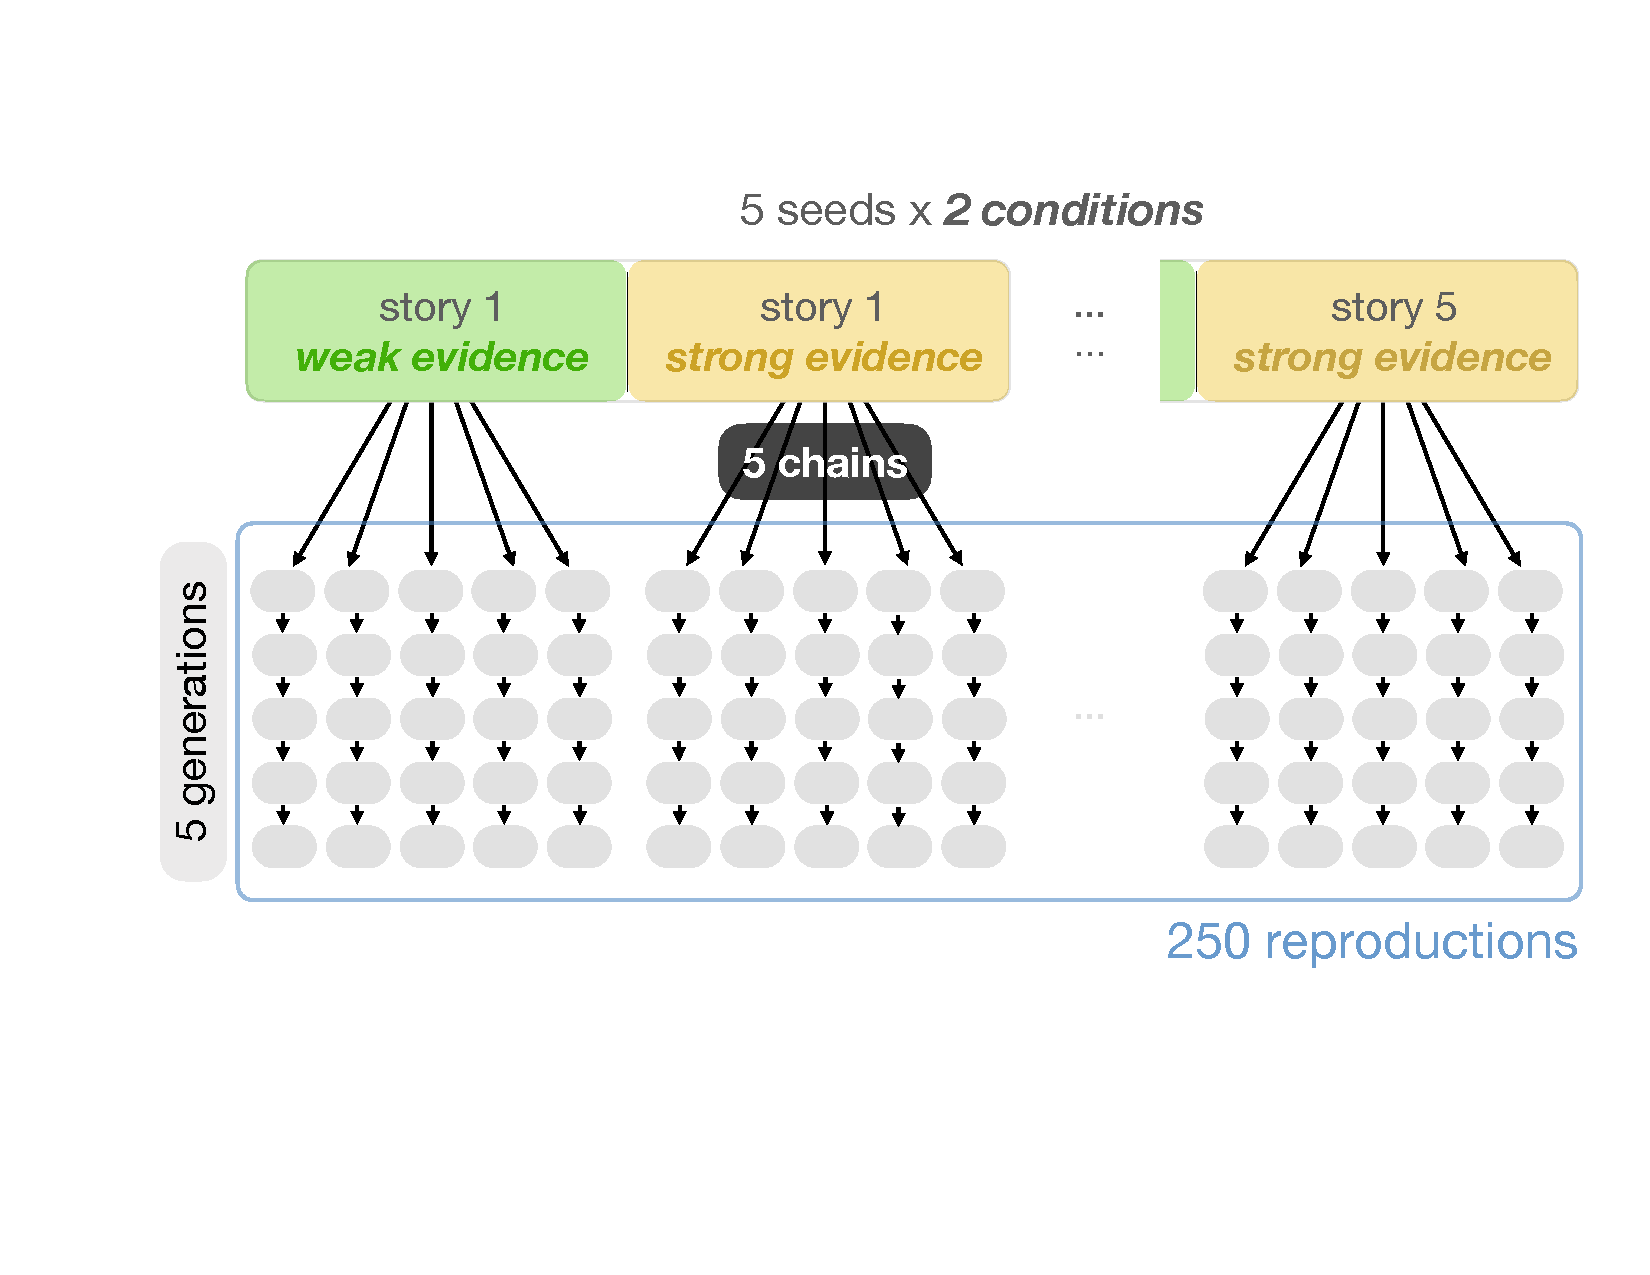
\includegraphics[width=\linewidth]{graphs/corpus-overview.pdf}
% 	\caption{Corpus collection schema as presented in \cite{Kreiss:2019}.}
% 	\label{fig:corpus-overview}
% \end{figure}

\begin{figure}[t!]
	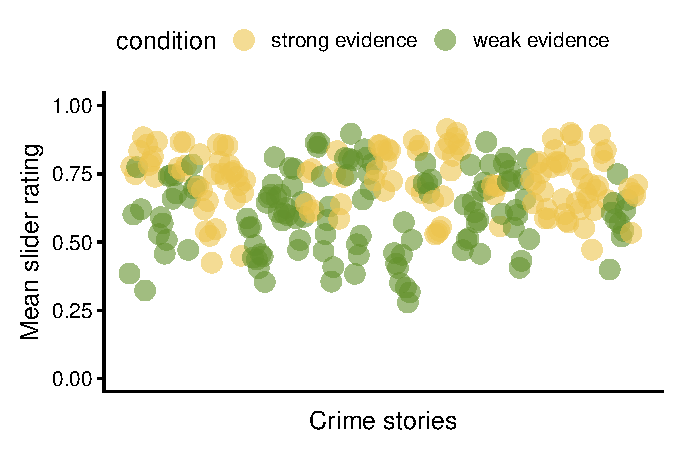
\includegraphics[width=\linewidth]{graphs/subjguilt.pdf}
	\caption{A point represents the mean subject guilt rating for a story in the corpus. They are color-coded with respect to their condition.}
	\label{fig:corpus-annotations}
\end{figure}

After the corpus collection, \citeauthor{Kreiss:2019} annotated the corpus with human judgments. The questions were primarily related to different aspects of guilt perception but also, for example, perceived subjectivity of the story writing. Participants were recruited on Amazon Mechanical Turk and indicated their response on a continuous slider, here underlyingly coded as ranging from 0 to 1. Most interestingly for this project, they asked ``How likely is it that the suspect is / the suspects in the crime are guilty?'' Each story received approximately 20 ratings, ranging from 0 to 1. For the purposes of this work, we consider the mean rating for each story as its guilt judgment label. The labels of each story are shown in Figure~\ref{fig:corpus-annotations}. In contrast to the raw ratings, the means only range from 0.27 to 0.92. 

% Subsequent analyses revealed that there are correlations with the number of hedges in the story, the length of the stories and of course with the evidence condition and therefore content expressed. 



In summary, the AINC is a corpus of reproduced news stories, annotated by human guilt judgments. Since the stories originated from only 5 unique stories (each in 2 conditions), a lot of information is shared between single data points.  Despite this similarity, the range of guilt judgments is still high, alluding to subtle differences that trigger this variance. We now turn to the question of whether a deep learning model can learn to predict the assessments of guilt the corpus provides.


% One of the challenges, this dataset poses, is its size. There are only 260 labeled examples that can be used for training and testing a model.
% Can a bidirectional LSTM with attention pick up on the patterns in human judgments with only very limited available data?

\section{Model}\label{model-architecture}

\begin{figure}[th]
  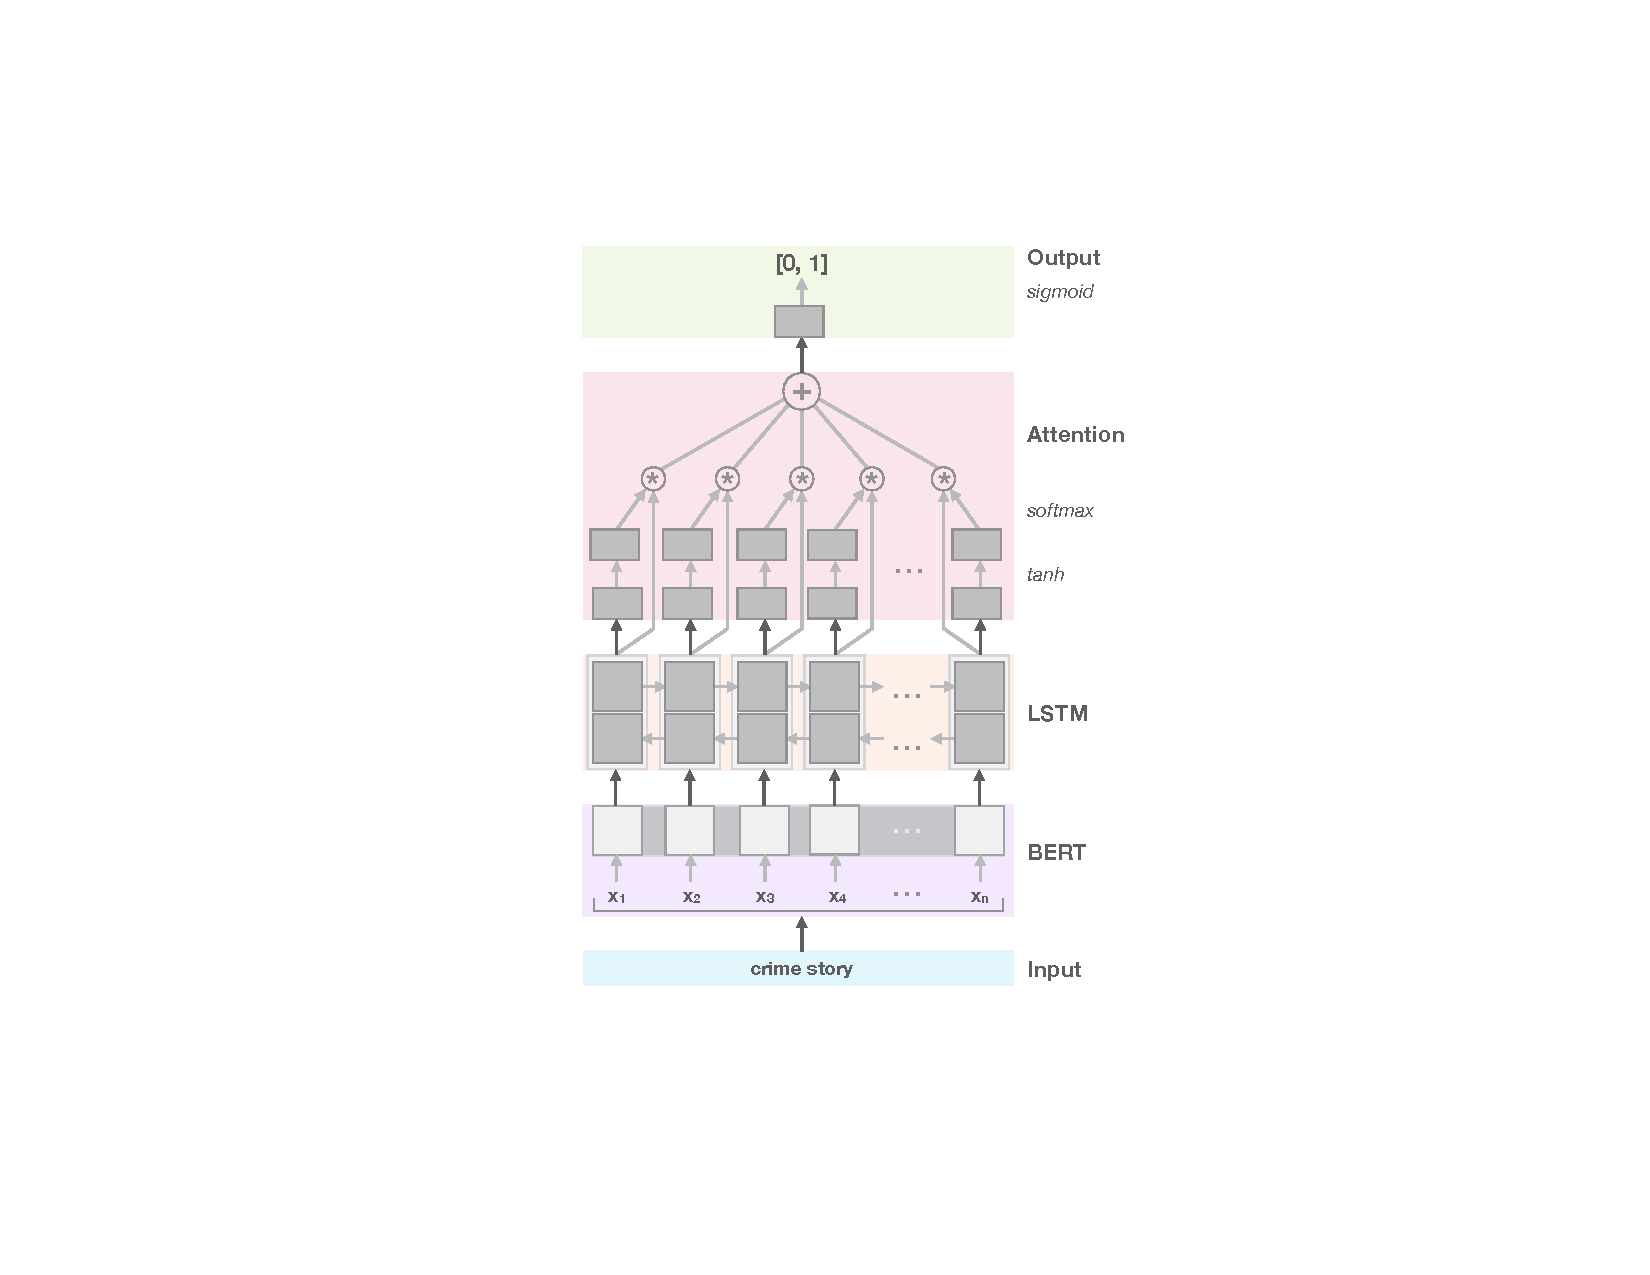
\includegraphics[width=1\linewidth]{graphs/model.pdf}
  \caption{Model architecture. The BERT layer produces
    a sequence of context-dependent representations. These
    are the inputs to the bidirectional LSTM, which
    fine-tunes these representations to our task.
    The LSTM outputs feed into the attention layer,
    which produces a summary representation of the full
    text that is weighted by each word's contribution
    to the final predictions.}
  \label{fig:model}
\end{figure}

Our model is based on the one proposed by \citeauthor{Lin:2017}, which is fundamentally a  bidirectional LSTM with attention mechanisms applied to its outputs. We chose this model primarily because its attention mechanisms seem especially promising for introspection, as they essentially provide a weight for each word in the input, and this weight controls how much each word contributes to the network's final predictions. The overall architecture is summarized in Figure~\ref{fig:model}.

% The goal of this work was to determine whether neural networks can be a useful tool to investigate the formation of guilt judgments. To do this, we used a model which was based on the design proposed by \citeauthor{Lin:2017}. We chose to use this model as our base because of its promising performances in various NLP tasks. Furthermore, its attention module provides a straightforward way to investigate the inner workings of the model.


The only major adjustment we made to the model is that we replaced the GloVe word embeddings \citep{Pennington:2014} by BERT representations \citep{Devlin:2018}. Whereas GloVe provides a single embedding for each word, with no sensitivity to the context in which it occurs, BERT representations vary by syntactic context. \citeauthor{Devlin:2018} report that using these embeddings boosts performance in all of the 11 natural language tasks they consider, and we saw comparable improvements when we switched from GloVe to BERT. To access pretrained BERT parameters, we used the Hugging Face toolkit.\footnote{\url{https://github.com/huggingface/pytorch-transformers}}

We allow BERT to tokenize the input string according to its internal tokenization method \citep{wu2016google}, to make maximal use of its own pretrained embedding. These token representations are processed by BERT using its pretrained Transformer parameters \citep{Vaswani:2017}, yielding a sequence of contextual representations for them. These are fed into a bidirectional LSTM layer in which each's cell's output has dimension $200$. The two representations at each step are concatenated to form the LSTM layer output for each token.

For the attention layer, we follow the design of \citeauthor{Lin:2017}: the LSTM outputs are organized into a matrix $H$ of dimension $n \times 400$, where $n$ is the token length of the current sequence, and we apply a dense layer with parameters $W$ (dimension $50 \times 400$) and a $\tanh$ activation to create a matrix $A$ of $50$-dimensional representations for each token:
\begin{equation}
  A = \tanh(WH^{\top}) \label{eq:A}
\end{equation}
%
The matrix $A$ is further compressed to the attention weight vector $\mathbf{a_w}$ of size $1 \times 50$, with a softmax applied so that the weights sum to 1:
%
\begin{equation}
  \mathbf{a_w} = \softmax(WA) \label{eq:attn}
\end{equation}
%
\citeauthor{Lin:2017} actually generalize this attention operation to return a matrix with $r$ attention weights for each token. We set $r=1$ to keep the number of parameters low and increase the interpretability of the network.

Finally, we take the dot product of the LSTM hidden state matrix $H$ and the just obtained vector $a_w$ to obtain the attention output vector $\aout$ of size $1 \times 400$:
%
\begin{equation}
  \aout = \mathbf{a_w}H \label{eq:aout}
\end{equation}
%
This is the output of the attention module. Intuitively, the attention weights capture the relative importance of each token with regard to the final prediction, and $\aout$ synthesizes all of these weighted contributions into a single vector.

Finally, the logistic regression module makes the prediction of guilt. For this step, $\aout$ is linearly transformed into a single number $p = \sigmoid(\aout)$. The sigmoid function ensures that the prediction lies between $0$ and $1$, just like the restriction on the guilt judgments it is trained on.

Overall, the model has $111,054,742$ trainable parameters. This sounds mismatched with our very small dataset, but only $0.02\%$ of these parameters are in the attention and output modules and $1.40\%$ are in the LSTM module. The rest of the parameters ($98.59\%$) are the pretrained weights in the BERT word embedding module.

In summary, the model receives a crime story as an input. BERT word embeddings for the story feed into a bidirectional LSTM. The attention module computes the weighted sum over the LSTM's hidden states. The resulting attention vector is fed through a linear layer and a sigmoid function to ensure that the prediction lies between 0 and 1.




\section{Experiment}

Our initial goal is to assess the extent to which our bidirectional LSTM with self-attention (as described in Section~\ref{model-architecture}) can predict human guilt judgments from news stories. Assuming the model succeeds, we can then probe its internal representations for linguistic insights.

\begin{figure*}
  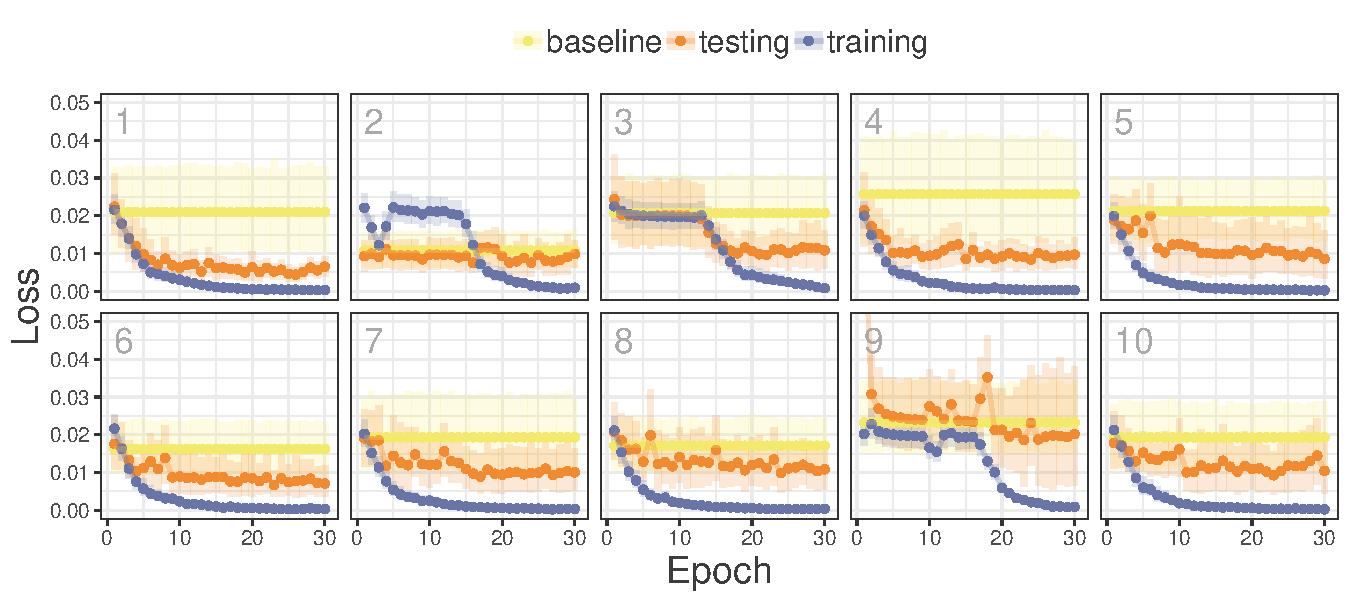
\includegraphics[width=\linewidth]{graphs/lossPlotCropped.pdf}
  \caption{Loss (mean squared error) over epochs (x axis), faceted over cross-validation configurations. The performance of the model on the training set (in blue) approaches zero. The performance of the model on the dev-test set (in orange) generally outperforms the baseline (in yellow).}
  \label{fig:loss}
\end{figure*}

\subsection{Optimization}

To begin with, we held out 26 randomly selected stories (from the 260 stories in total) as the final test set. The remaining 234 stories were then used for model training and validation, which was done using 10-fold cross validation. The cross-validation results inform us about the model variation observed across  various training/validation splits; it is quite likely that, given the small size of the dataset, this variation could be quite high.

In each step of the 10-fold cross-validation, the model was trained on 206/207 stories and 23/24 were held out for dev-testing. As noted above, this guilt rating is the mean participant guilt rating obtained from the previously described data collection and annotation.

For training, the model uses mean squared error (MSE) as the loss function, stochastic gradient descent as the optimizer, and a learning rate of 0.1. The model was implemented using PyTorch \citep{Paszke:2017}. It was trained for 30 epochs, for each of the 10 training/dev-test configurations in the cross-validation.

%From the 260 stories with their respective mean suspect guilt rating, 26 were randomly held back as a final testing set. The guilt rating is the mean obtained from the previously described data collection and annotation. Crucially, the target values range between 0 and 1, which is why the model does not learn a classification, but regression task. The remaining 234 stories were used for training the model. 

%To assess the model performance during development, we need to exclude more stories from training to be able to use them as dev-testing data. To make the most use of the limited amount of data, the model was trained using 10-fold cross-validation. The results can also inform us, whether there is strong variation given a different training/dev-testing split. It is very likely that given the small size of the dataset (and therefore dev-test set), the variation can be quite high. Given that there were 234 stories for training, each fold had between 23 and 24 stories, each associated with one guilt rating that functioned as the target label. 


\subsection{Results}

Figure~\ref{fig:loss} shows the MSE loss for each training epoch. We show the dev-set loss for our model (orange) as well as the train-set loss (blue). In addition, to provide context for the results, we include the loss for a dummy regressor that simply predict the mean of the training data labels for all cases.

The training loss approaches 0 toward the end of the training in all cross-validation configurations, indicating model convergence. Crucially, our model's dev-set performance is always subtantially better than the baseline model, indicating that the model is indeed learning from the dataset. That said, there is a high amount of variation between the different cross-validation steps, with the baseline actually proving competitive in some folds. This seems an inevitable consequence of our small dataset, but the model clearly has gotten traction on the problem overall.

% The mean of the training labels alone (i.e., the baseline) only has a very small loss on cross-validation configuration 2 and the trained model can barely beat it. This is in clear contrast to cross-validation step 4, where the baseline model loss is very high on the dev-test data and the trained model can easily surpass it. Those two cases exemplify the high variation that comes with the different splits of training and dev-testing data\footnote{However, I cannot exclude that also the random parameter initialization plays a relevant role here. But at least the differences in the baseline are definitely caused by the different splits.}.

The MSE loss alone is not sufficient to assess how well the model actually learns to predict the underlying distribution. Figure~\ref{fig:corr-cv0} shows the correlation between the actual target labels (on the x axis) and the model predictions (on the y axis) for one of the cross-validation folds. Before training (left), the models are undifferentiated. After training (right), the model predictions (blue) are highly correlated with the true labels ($r=0.85$), and the MSE is small ($0.007$).

Qualitatively, these plots appear very similar throughout all cross-validation configurations and can be compared in Figure~\ref{fig:app-corr-pretraining} and \ref{fig:app-corr-posttraining} in the Appendix. Quantitatively the correlation on the dev-test set does show variation, driven mainly by outliers.\footnote{\ek{Note on professor seed as outlier: Story about sexual harrassment allegations against male professor; only story that has clear gender split between victim(s) and suspect; Erickson 1978 show that powerless style (which includes hedges) affects credibility ratings dependent on whether witness is same or other sex}} However, overall, the mean correlation between the model prediction and the human judgment on the testing set across all cross-validation steps is $0.68$. When we collapse over all cross-validation folds and examine the loss after training, the difference in loss between the model predictions and baseline is significant ($p<0.0001$).\cp{Which test was used to get this p-value?}

As a final performance evaluation, we examine the target--prediction correlation on the held-out test set (Figure~\ref{fig:test-corr}). For predictions on the test set, we used the final model weights obtained by the first cross-validation configuration. This setup was chosen because of the low dev-set loss and the high correlation of the dev-set with the target labels. This was the only evaluation that was performed on this held-out test set. The Pearson correlation on the held-out test set is still high ($0.84$) and almost identical with performance on the dev-set for this fold. This high correlation, and the fact that the high correlation reproduces with the held-out testing data, indicates that the model was able to learn to generalize.

\begin{figure}
  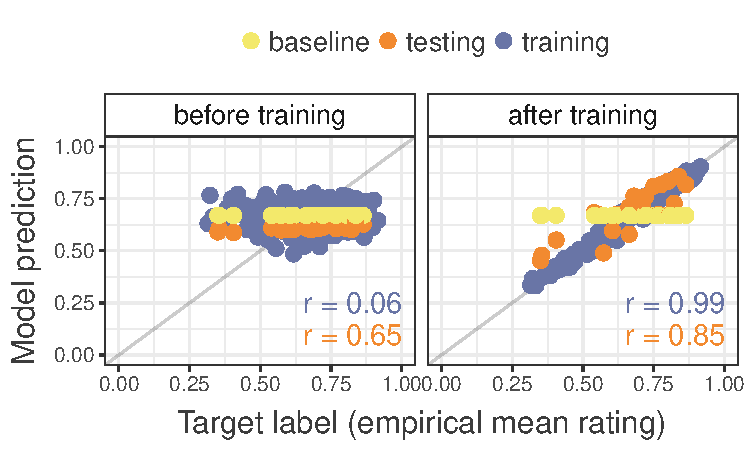
\includegraphics[width=\linewidth]{graphs/cv0-pred-target-epoch0-29.pdf}
  \caption{Correlation between target label (x axis) vs. model prediction (y axis) before and after training.}
  \label{fig:corr-cv0}
\end{figure}

\begin{figure}
  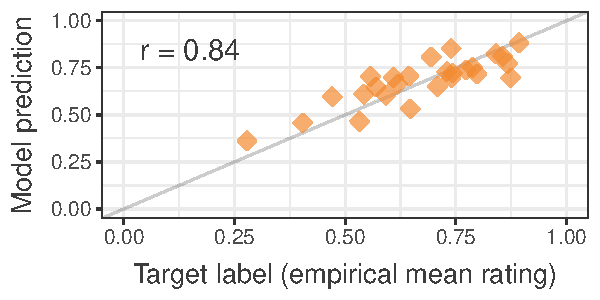
\includegraphics[width=\linewidth]{graphs/test-corr.pdf}
  \caption{Testing label (x axis) vs. model prediction (y axis) after training on the held out test set (26 data points) using the parameter settings obtained after the 30th epoch from the first cross-validation. Pearson correlation of 84\%.}
  \label{fig:test-corr}
\end{figure}


\section{Model analysis}

We have established that the proposed model can predict human guilt judgments when given a crime story. This result invites us to ask the question of whether there are patterns underlying these predictions that can provide higher-level insights into how langauge is construed in these criminal contexts. 

\begin{figure*}[t]
  \centering
  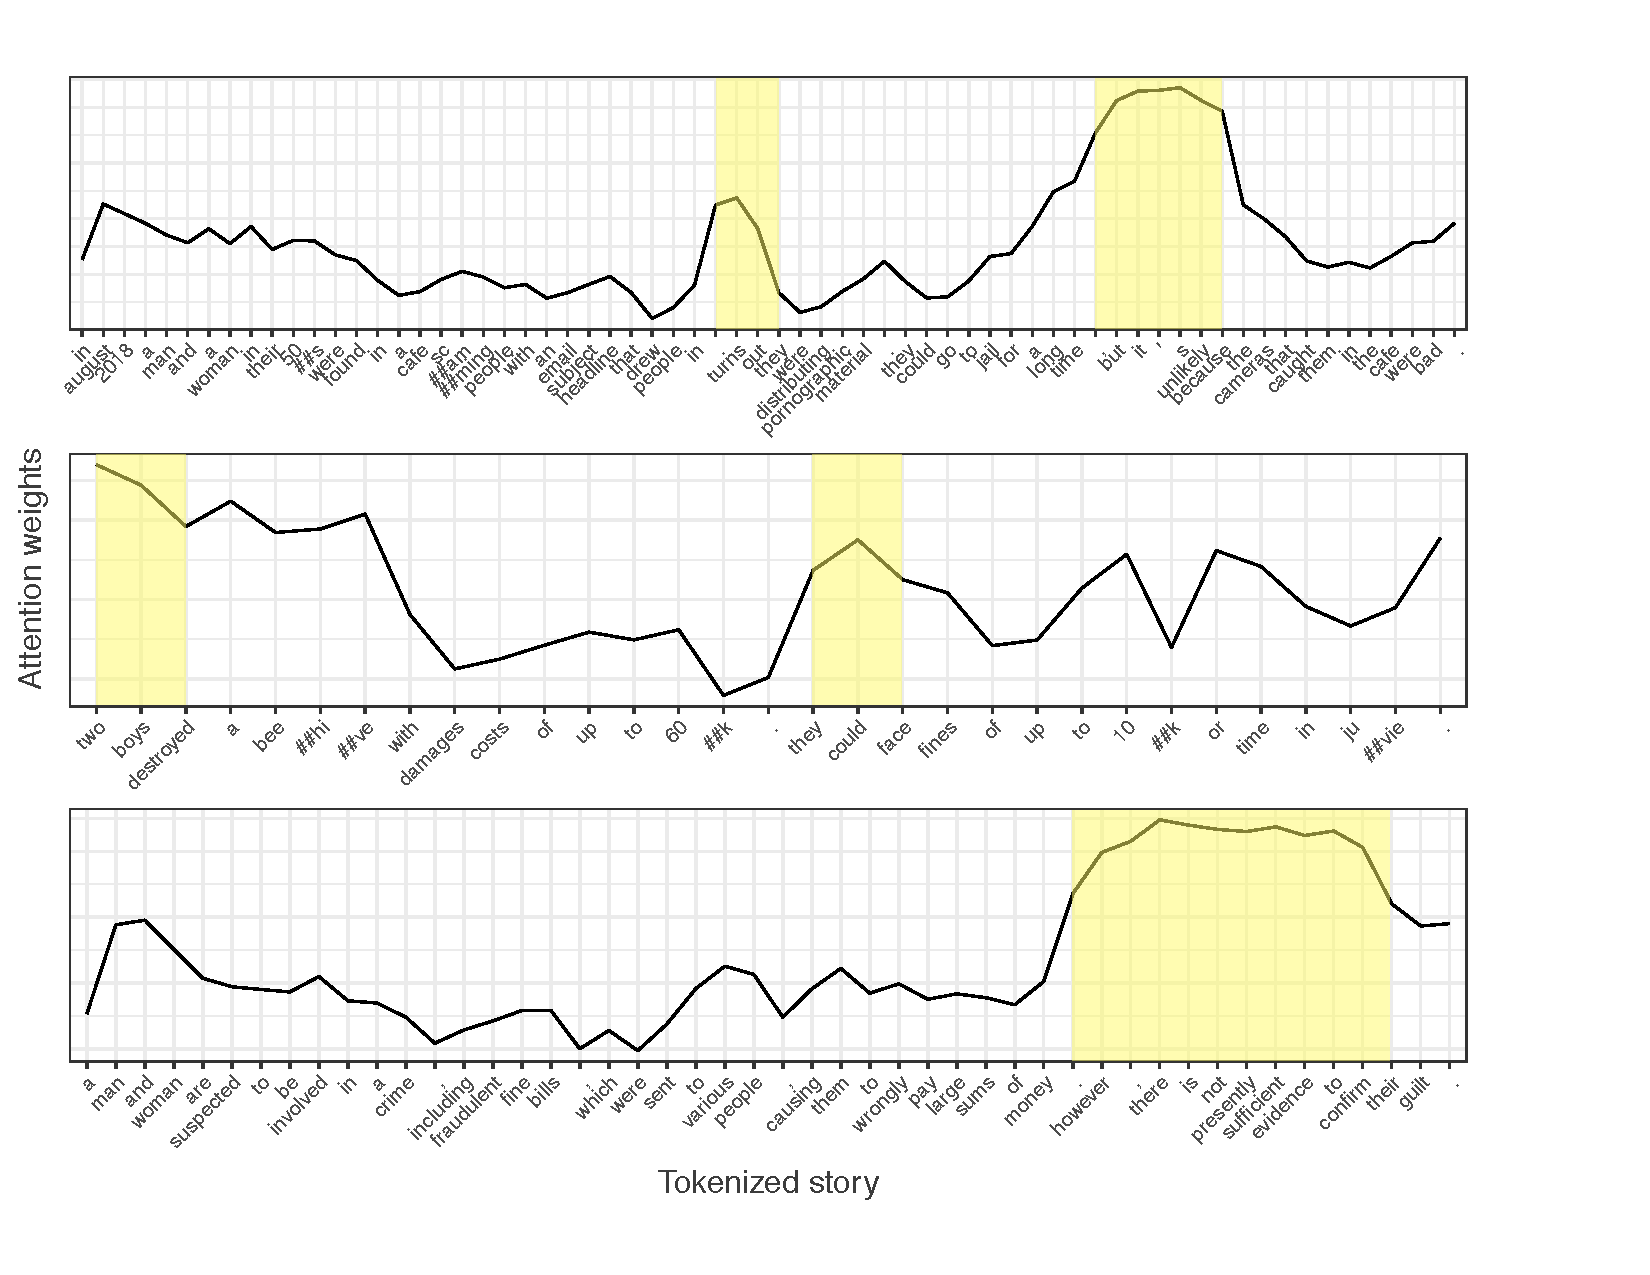
\includegraphics[width=1\linewidth]{graphs/attention-marked.pdf}
  \caption{Visualization of the attention weights (y axis) for a tokenized story (x axis) from the test set. Because we took the softmax over the attention weights, the scale of the y axis is irrelevant. Areas of high attention weight are marked in yellow and correlate with markers of (un)certainty as well as markers of contrast. \cp{The panel needs A, B, and C marks. I thought about adding them to the PDF image, but there isn't really room in it.}}
  \label{fig:viz}
\end{figure*}

\subsection{Visualization}

We begin by focusing attention on the learned attention weight vector $\mathbf{a_{w}}$ in equation (\ref{eq:attn}). Since the softmax forces the sum of the weights to be 1, we cannot interpret the weights on their own for each word or across stories. Instead, the relevance lies in the differences between words and phrases within each story, and patterns of similarities between stories.

To investigate what might affect model predictions, we ran the model again on the final test data. Figure~\ref{fig:viz} displays three of these stories with their attention weight distribution.
We see that the model seems to focus on phrases that explicitly describe uncertainty about the evidence (see Figure~\ref{fig:viz}C). If present, these cues usually outweigh the rest of the story. This suggests that, if there is an explicit claim that affects the evidence of the suspect's guilt, it is considered as the most important source to inform guilt judgment.

Additionally, peaks occur on words and phrases which communicate turning points in a story, such as ``however'', ``but'', ``even though'', and ``it turns out''. This can be seen in all three stories in Figure~\ref{fig:viz}. Those phrases could be relevant because they usually indicate a contrast to a prior narrative. Since those markers mostly follow reports of arrests, they might be strongly correlated with objections to those arrests which would in turn influence guilt perceptions.

Figure~\ref{fig:viz}B shows a case where the model seems to find a simple declarative (``two boys destroyed'') to be relevant for the final prediction. This is especially interesting, since declaratives on their own do not generally communicate guilt-related information. However, they are very important for guilt judgments because they do not allow any uncertainty about the association between crime and suspect.

In summary, the visualization of the attention weights contribute further evidence that the model learns meaningful patterns in the data.


\subsection{Qualitative Analysis}

Figure~\ref{fig:viz} provides evidence for the claim that the model picks up on meaningful patterns in the corpus. But does the model make reasonable predictions on newly constructed data points?  The original corpus started out with five different crime stories. Each of these stories occurred in two conditions -- one suggesting that the evidence that led to the arrest was weak, and the other that the evidence provided a strong case. Additionally, the stories were filled with uncertainty markers such as ``allegedly'' or ``(un)likely'', which we expect to have an impact on guilt judgments. Howver, the corpus cannot inform us about this relationship.

\begin{figure}
	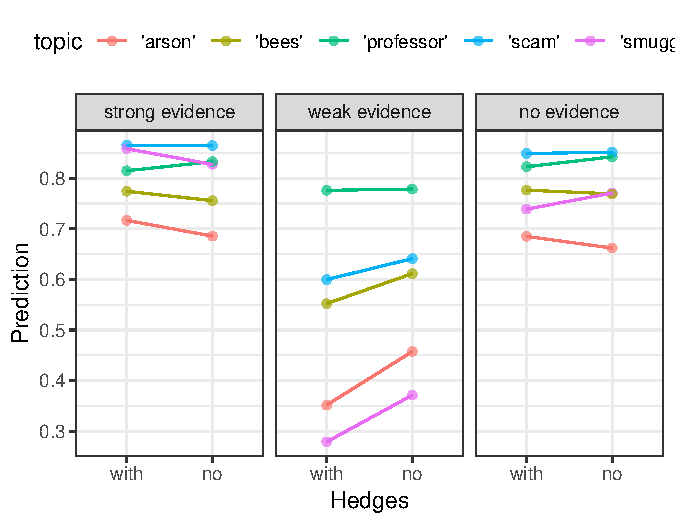
\includegraphics[width=1\linewidth]{graphs/hedges.pdf}
	\caption{Model predictions on the relationship between uncertainty markers and evidence statements. \ek{fix caption and make figure more readable}}
	\label{fig:hedges}
\end{figure}


We can, though, use the model to predict a guilt judgment for each of the original stories without these uncertainty markers/hedges. Thus, we rewrote those 10 original stories into versions without any uncertainty markers. They remained as close to the original as possible, while still remaining grammatical.
Figure~\ref{fig:hedges} summarizes this analysis. The results suggest that uncertainty markers have different effects on guilt prediction in the two evidence conditions. When the evidence is strong, removing all uncertainty markers does not affect the guilt judgments. However when the evidence is weak, removing those hedges increases the guilt judgment. This has an intuitive interpretation: when evidence already overwhelmingly speaks for the suspect's guilt, it outweighs the hedges; when  the evidence is questionable, other sources of uncertainty are considered to inform a final judgment.

Notably, if the evidence manipulation is excluded, the model predicts guilt judgments in the range of the strong evidence condition. In other words, the model assumes that additional justification for an arrest does not change the model's prediction of a guilty judgment. However, if reasons to question the arrest are given explicitly, this does affect the model's prediction. When we remove the hedges again, we cannot see a common structure to the change in ratings (possibly more similar to the strong evidence ratings though).\cp{I am not sure I understand this last sentence. Could it be expanded?}

% I think we don't need a separate section for this. Better to just ensure that
% the previous section ends in a clear and strong way.
%
% \subsection{Conclusion}
%
% In this section we showed that our attention module provides intuitive insight into the model workings. Furthermore, the model makes interesting predictions on new data.\ek{...}

\section{Discussion}
\ek{past tense!}
The way a crime and arrest is presented in a news article affects how readers perceive the suspect's guilt. In this paper we showed that a recurrent neural network with self-attention can predict readers' guilt judgments. 
By visualizing the attention weights, we find that explicit evidence descriptions and phrases suggesting a turn of events influence predictions. 

To gain linguistic insights into the neural network, we investigated its change in predictions when we exclude the hedges and information about the evidence from the stories. First of all the model makes similar predictions in the case where the evidence leading to an arrest is strong/convincing and the case where the evidence is not specified. 
\ek{One possible interpretation of this result is that the model learns that there is an implicature of strong evidence if the evidence is underspecified?} The model predictions are affected the most when the weakness of the evidence is mentioned explicitly.

Furthermore, we found that an exclusion of hedges in the stories only seems to affect predictions of stories in the weak evidence condition, where suspects are rated more guilty when there are no hedges. However, if the evidence is strong or underspecified, the model predictions do not seem to be affected. 
Possibly, in case of strongly perceived evidence, the model has learned that the hedges become irrelevant.

These results point to promising avenues for future investigations of hedging, particularly in the field of guilt perception. 

\ek{how we perceive stories affects how we reproduce them; relevance for iterated chains}



\ek{Conclusion: propose a network that can predict guilt judgments and might be used to inform hypotheses for insight on linguistic features that determine guilt perception...}



% Commenting these out now so that we don't accidentally include them in the submission,
% which has to be anonymous.
%\section*{Acknowledgments}

%I'm particularly thankful for the valuable feedback from Sebastian Schuster. \ek{any grants to cite here, Judith?} \\


\bibliography{acl2019}
\bibliographystyle{acl_natbib}

\onecolumn
\section{Appendices}
\label{sec:appendix}

\begin{figure*}[!htb]
	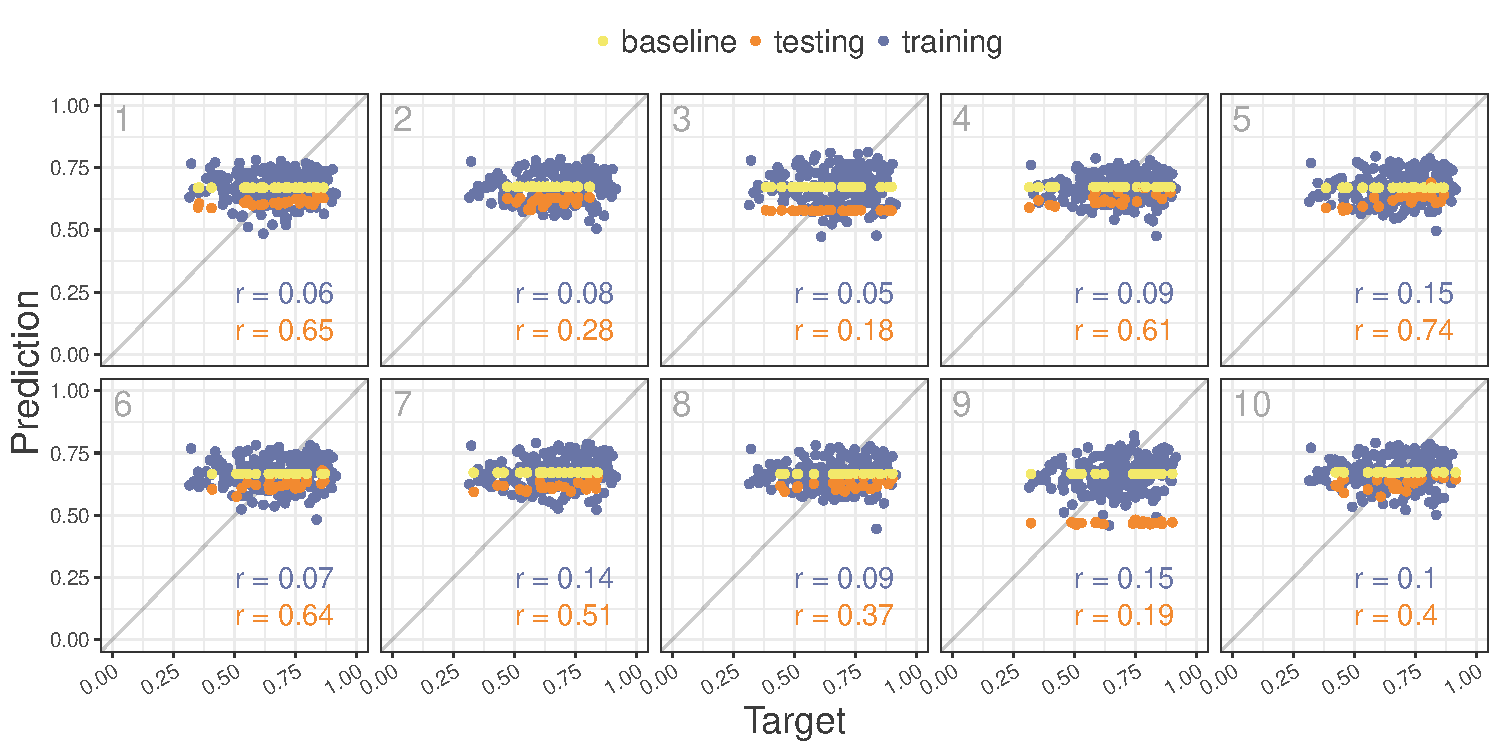
\includegraphics[width=\linewidth]{graphs/all-pred-target-epoch1.pdf}
	\caption{Testing label (x axis) vs. model prediction (y axis) before training; faceted over cross-validation configurations.}
	\label{fig:app-corr-pretraining}
\end{figure*}

\begin{figure*}[!htb]
	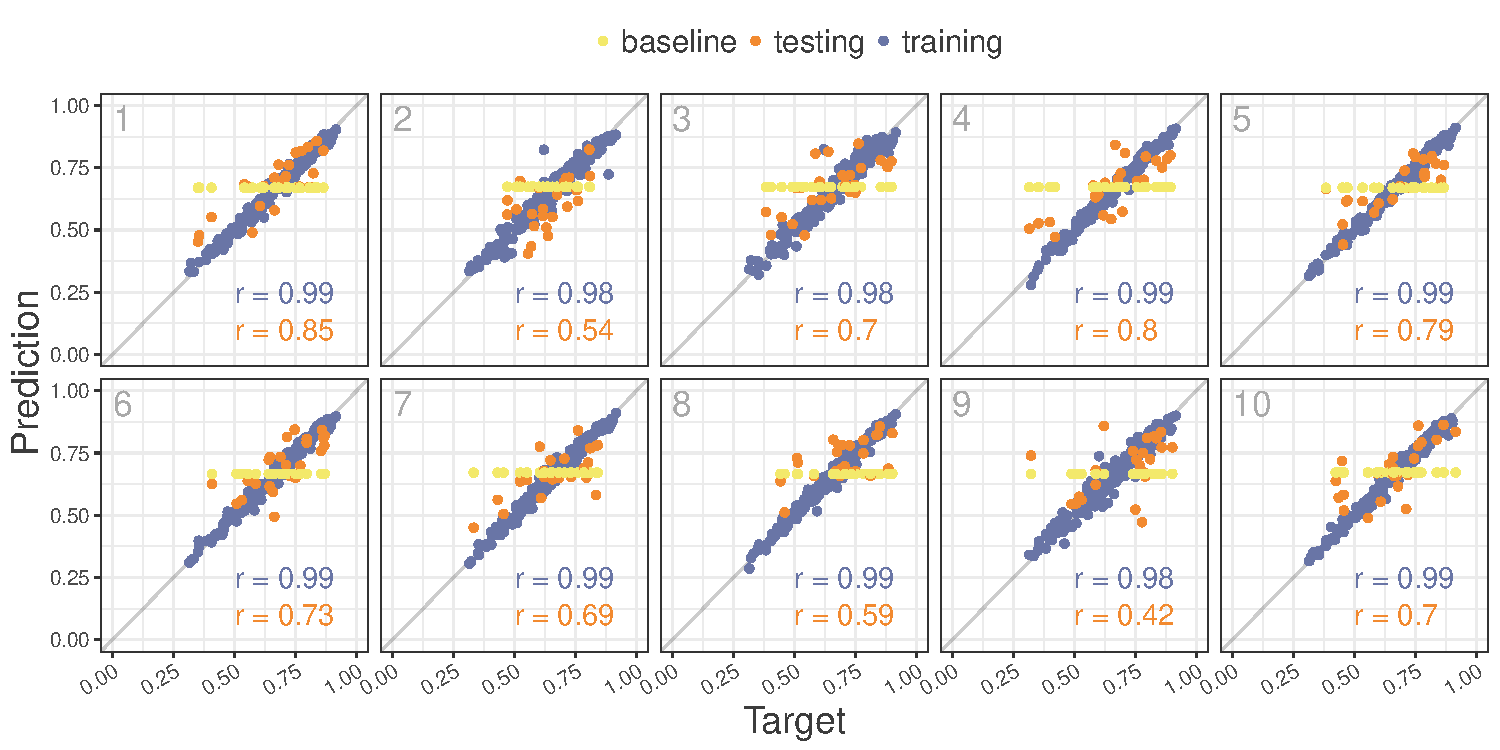
\includegraphics[width=\linewidth]{graphs/all-pred-target-epoch30.pdf}
	\caption{Testing label (x axis) vs. model prediction (y axis) after training; faceted over cross-validation configurations.}
	\label{fig:app-corr-posttraining}
\end{figure*}

\end{document}
